\documentclass{standalone}
\usepackage{tikz}
\usetikzlibrary{calc}
\usepackage{amssymb}

\begin{document}

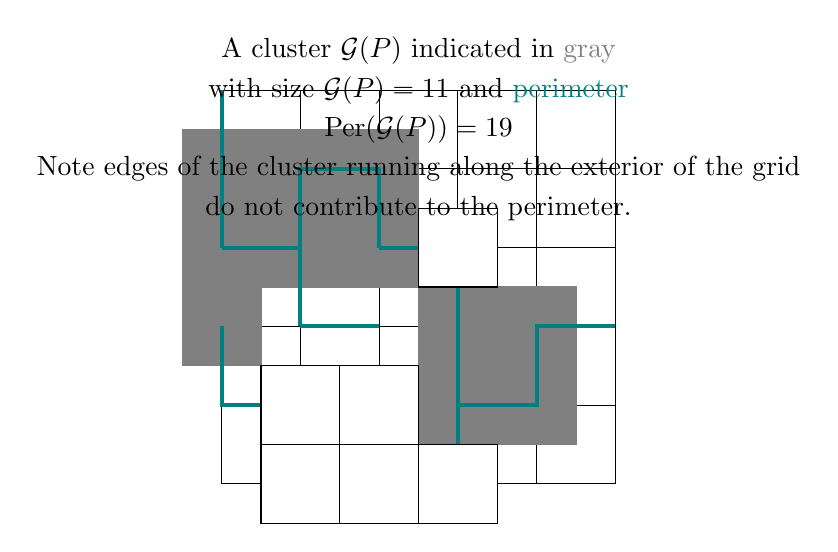
\begin{tikzpicture}
    % Grid lines
    \draw[step=1cm, color=black] (0,0) grid (5,5);
    
    % Gray squares
    \foreach \pos in {(0,4), (1,4), (2,4), (0,3), (1,3), (2,3), (3,2), (4,2), (0,2), (3,1), (4,1)} {
        \node[rectangle, fill=gray, minimum size=1cm, draw=gray, outer sep=0] at \pos {};
    }
    
    % Perimeter edges in teal
    \draw[teal, line width=0.5mm] 
        (0,4) -- (0,3) 
        (0,3) -- (1,3) 
        (1,3) -- (1,2) 
        (1,2) -- (2,2) % Middle of grid down
        (1,3) -- (1,4) -- (2,4) -- (2,3)
        (2,3) -- (3,3) -- (3,2) -- (3,1) -- (4,1) -- (4,2) -- (5,2) % To the right
        (0,4) -- (0,5) % Top edge
        (0,2) -- (0,1) -- (1,1) -- (1,0) % Down left
        (3,1) -- (3,0); % Down right
    
    % White squares (explicitly place to ensure clarity)
    \foreach \pos in {(1,1), (2,1), (3,3), (1,0), (2,0), (3,0)} {
        \node[rectangle, fill=white, minimum size=1cm, draw=black, outer sep=0] at \pos {};
    }
    
    % Annotations
    \node at (2.5, 5.5) {A cluster $\mathcal{G}(P)$ indicated in \textcolor{gray}{gray}};
    \node at (2.5, 5) {with size $\abs{\mathcal{G}(P)} = 11$ and \textcolor{teal}{perimeter}};
    \node at (2.5, 4.5) {$\mathrm{Per}(\mathcal{G}(P)) = 19$};
    \node at (2.5, 4) {Note edges of the cluster running along the exterior of the grid};
    \node at (2.5, 3.5) {do not contribute to the perimeter.};
\end{tikzpicture}

\end{document}